\section{Аналитический раздел}

\subsection{Формализация задачи}

Требуется разработать базу данных приложения по организации археологических экспедиций. В базе будет храниться информация об экспедициях, руководителях, кураторах и участниках экспедиций, местах раскопок, найденных там артефактах и необходимом для экспедиций снаряжении. Также необходимо разработать интерфейс для взаимодействия с базой данных. 

Необходимо предусмотреть возможность создавать экспедиции с указанием
места проведения, временных рамок, кураторов, руководителей и участников. 
Требуется реализовать три вида ролей --- участник экспедиции, руководитель и администратор. Реализовать возможность для пользователя просматривать, создавать экспедиции и добавлять других участников в зависимости от его роли.

\subsection{Формализация данных}
База данных должна содержать информацию о следующих сущностях:

\begin{enumerate}[left=0.49cm, label*=---]
        \item экспедициях;
        \item руководителях экспедиций;
	\item участниках экспедиций;
	\item местах проведения экспедиций;
        \item кураторах экспедиций;
        \item снаряжении для экспедиций;
        \item найденных артефактах.
\end{enumerate}

В таблице \ref{tab:types} приведены данные сущности и сведения о них.
\newpage

\begin{table}[hbtp]
	\begin{center}
			\caption{\label{tab:types}Сущности и сведения о них}
		\begin{tabular}{|l|l|l|l|}
			\hline {Сущность} & {Сведения}  \\ \hline
            Локация & \begin{tabular}[c]{@{}l@{}}ID локации, название, страна, ближайший населенный\\ пункт\end{tabular} \\ \hline
			 Экспедиция & \begin{tabular}[c]{@{}l@{}}ID экспедиции, ID локации, дата начала экспедиции,\\ дата окончания экспедиции\end{tabular} \\ \hline
            Участник & \begin{tabular}[c]{@{}l@{}}ID участника, имя, номер телефона, роль в экспедиции,\\ логин, пароль \end{tabular} \\ \hline
            Руководитель & \begin{tabular}[c]{@{}l@{}}ID руководителя, имя, номер телефона, логин, пароль \end{tabular} \\ \hline
            Куратор & \begin{tabular}[c]{@{}l@{}}ID куратора, название \end{tabular} \\ \hline
            Снаряжение & \begin{tabular}[c]{@{}l@{}}ID снаряжения, ID экспедиции, название, количество\end{tabular} \\ \hline
            Артефакт & \begin{tabular}[c]{@{}l@{}}ID артефакта, ID локации, название, возраст\end{tabular} \\ \hline
		\end{tabular}
	\end{center}
\end{table}

На рисунке \ref{img:ER} представлена ER-диаграмма сущностей проектируемой базы данных в нотации Чена.

\begin{figure}[!h]
	\centering
	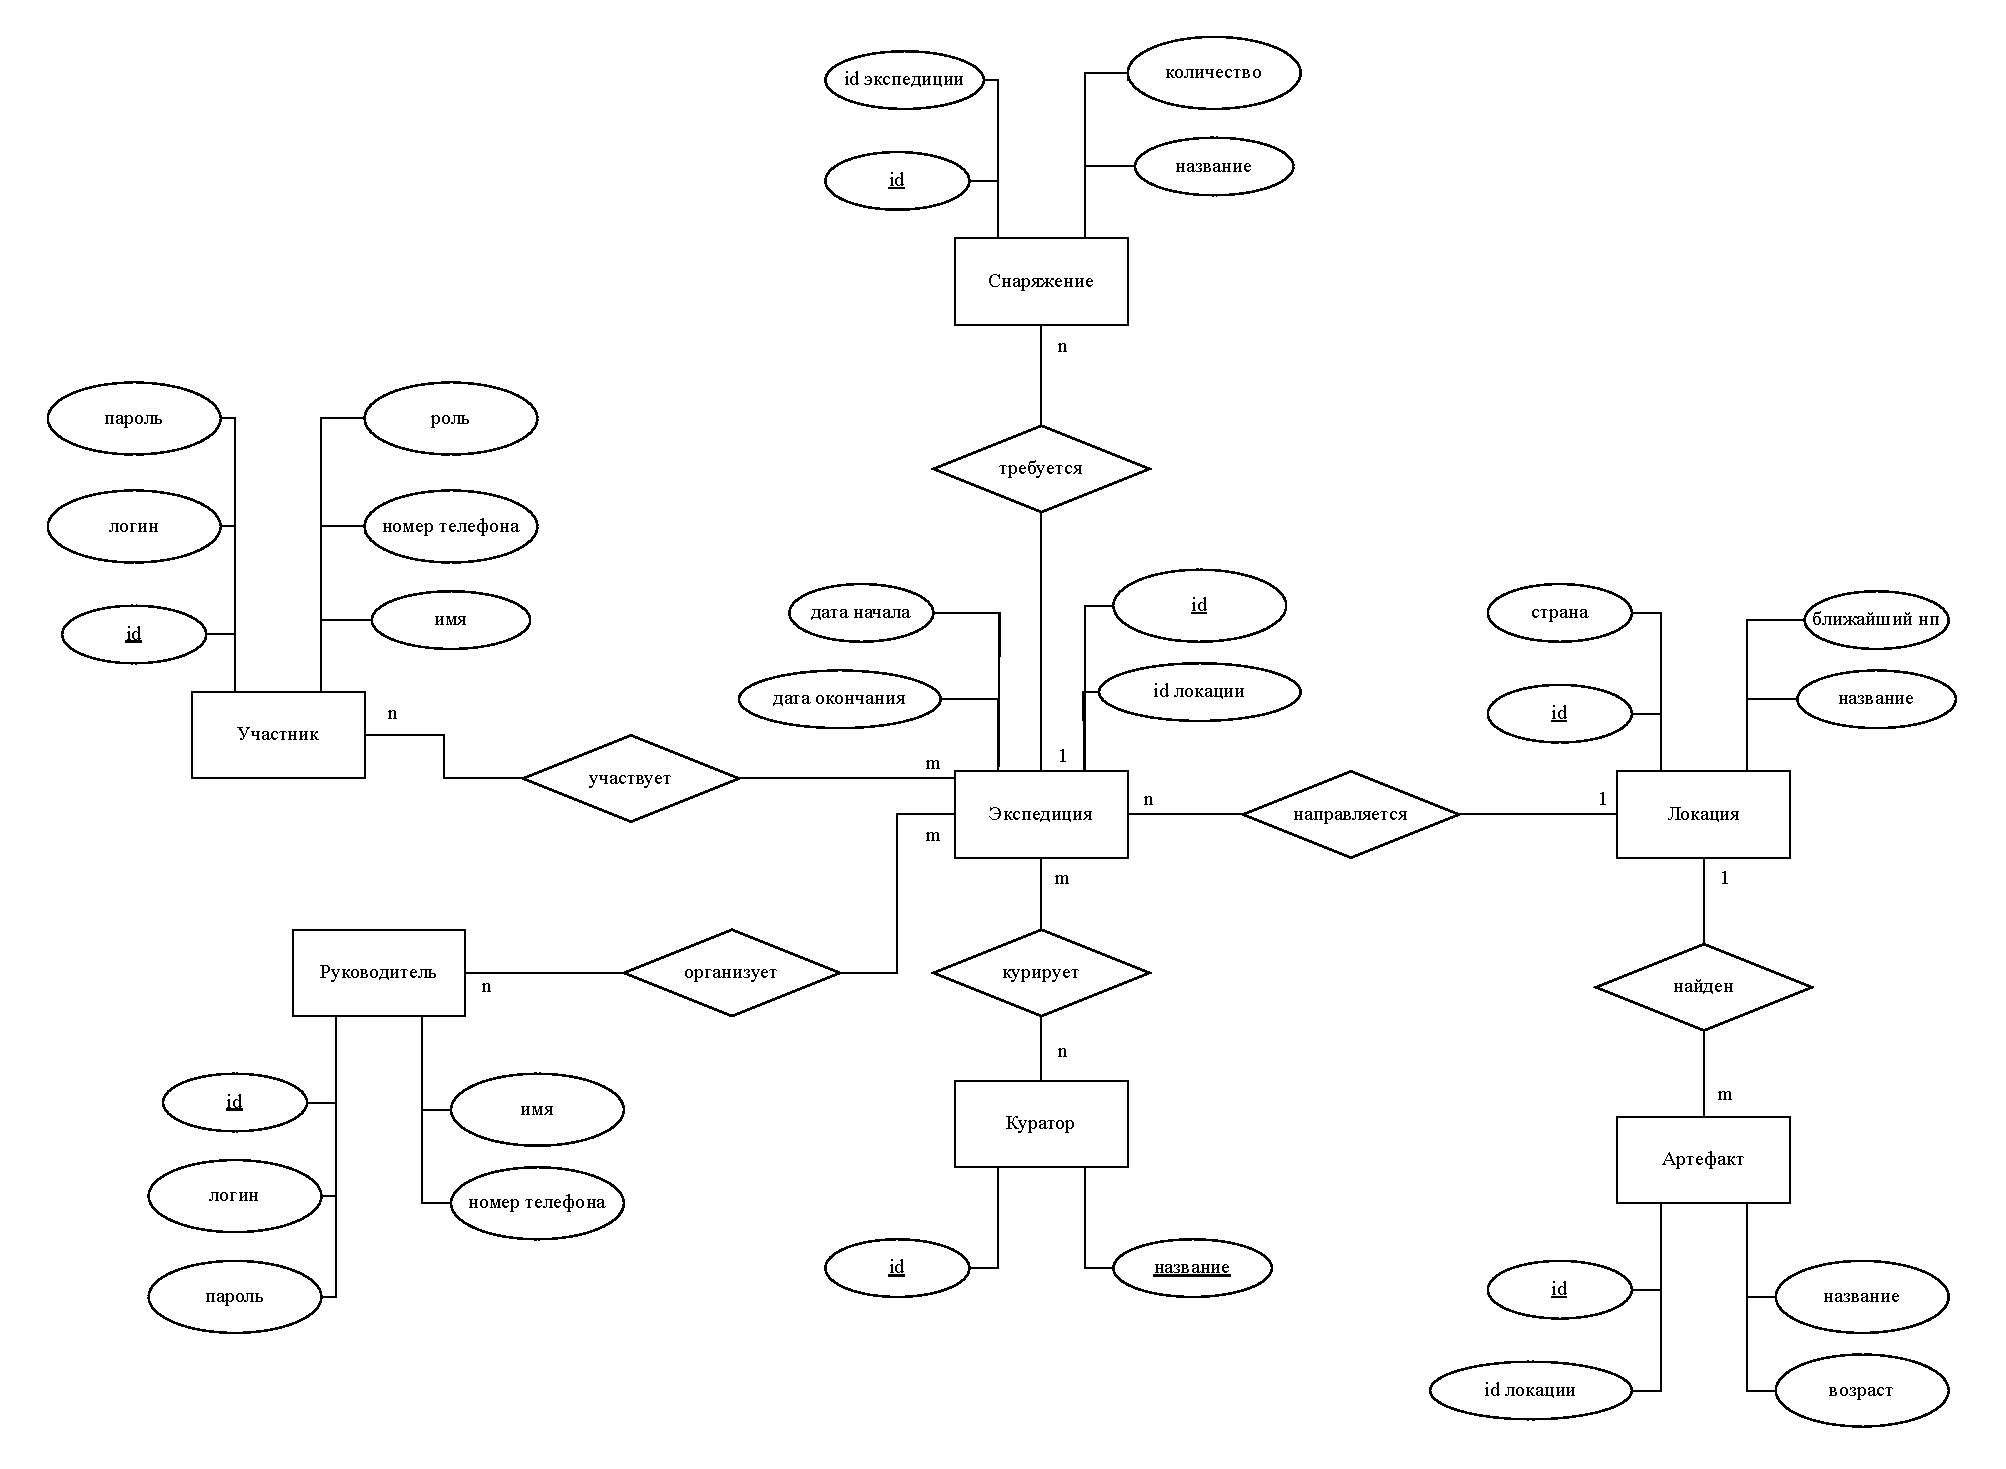
\includegraphics[width=\textwidth]{image/ER.pdf}
	\caption{ER-диаграмма}
	\label{img:ER}
\end{figure}
\newpage


\subsection{Формализация ролей}
Для управления приложением выделено три типа пользователей: участник экспедиции, руководитель и администратор. Для каждой роли предусмотрен свой набор функций.

Набор функций участника:

\begin{enumerate}[left=0.49cm, label*=---]
        \item выйти из аккаунта;
        \item просмотр информации об экспедициях;
        \item просмотр информации о руководителях экспедиций;
        \item просмотр информации об участниках экспедиций;
        \item просмотр информации о кураторах экспедиций;
        \item просмотр информации о местах проведения экспедиций;
        \item просмотр информации о найденных артефактах;
        \item просмотр информации о снаряжении для экспедиций.
\end{enumerate}

Набор функций руководителя:

\begin{enumerate}[left=0.49cm, label*=---]
        \item все возможности роли <<участник>>;
        \item добавление и удаление информации об участниках экспедиций;
        \item добавление, изменение и удаление информации об экспедициях;
        \item добавление и удаление информации о кураторах экспедиций;
        \item добавление и удаление информации о местах проведения экспедиций;
        \item добавление информации о найденных артефактах;
        \item добавление и удаление информации о снаряжении для экспедиций.
\end{enumerate}

Набор функций администратора:

\begin{enumerate}[left=0.49cm, label*=---]
        \item все возможности роли <<руководитель>>;
        \item добавление и удаление информации о руководителях экспедиций.
\end{enumerate}

Диаграмма вариантов использования приложения для выделенных ролей представлена на рисунке \ref{img:use-case}.

\begin{figure}[!h]
	\centering
	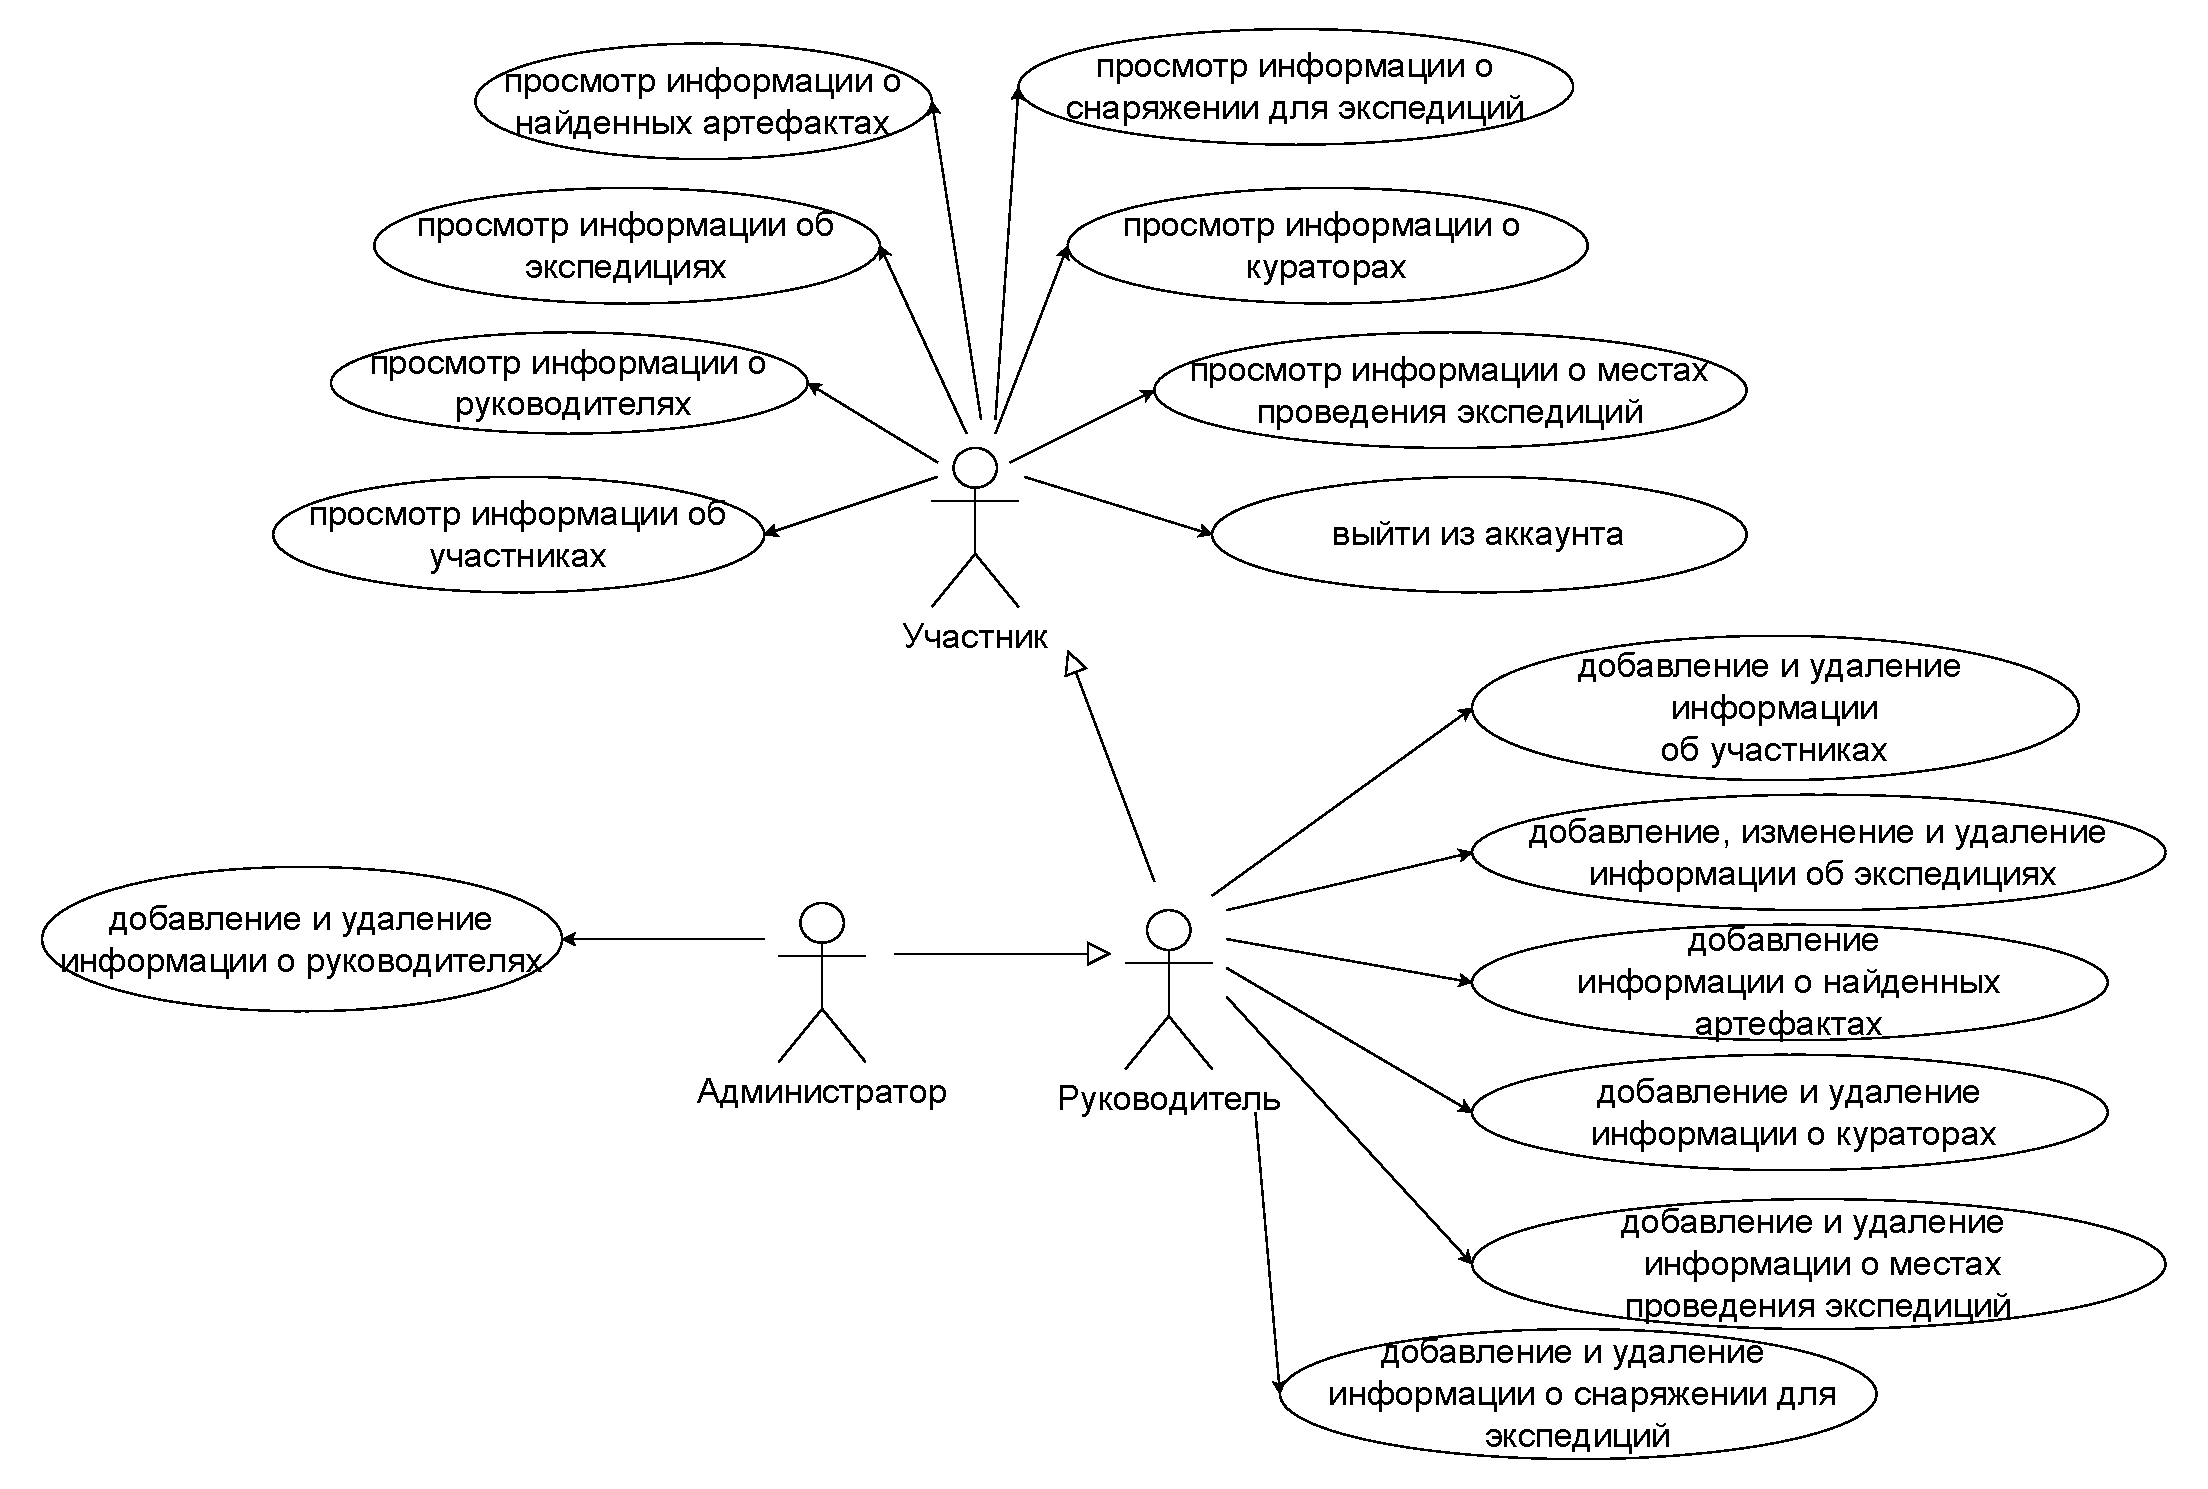
\includegraphics[width=\textwidth]{image/use-case.pdf}
	\caption{Диаграмма вариантов использования}
	\label{img:use-case}
\end{figure}
\newpage


\subsection{Базы данных и системы управления базами данных}

База данных --- это упорядоченный набор структурированной информации или данных, которые обычно хранятся в электронном виде в компьютерной системе~\cite{db}.

Для базы данных обычно требуется комплексное программное обеспечение, которое называется системой управления базами данных (СУБД).
СУБД основываются на различных моделях данных, которые определяют, каким образом данные будут храниться и обрабатываться внутри СУБД.
Существуют три основных типа моделей данных, отличающиеся структурой организации данных --- дореляционные, реляционные и постреляционные.

\subsubsection{Дореляционные}
Ранние модели называются дореляционными~\cite{before}. К ним относятся следующие модели.

\begin{enumerate}[left=0.49cm, label=\arabic*.]
        \item Инвертированные списки (файлы).
	\item Иерархическая.
	\item Сетевая.
\end{enumerate}

База данных на основе инвертированных списков представляет собой совокупность файлов, содержащих записи (таблиц). Для записей в файле определен порядок, диктуемый физической организацией данных. На основе инвертированных списков для каждого файла может быть определено произвольное число других упорядочений.

Иерархическая модель состоит из объектов с указателями от родительских объектов к потомкам, соединяя вместе связанную информацию. Такие базы данных могут быть представлены как дерево.

К основным понятиям сетевой модели относятся: элемент (узел) и связь.
Узел представляет собой совокупность атрибутов данных, описывающих некоторый объект. Сетевая база данных может быть представлена в виде графа. Сетевая модель не является полностью независимой от приложений, так как логика выборки данных зависит от физической организации этих данных~\cite{before2}. 

\subsubsection{Реляционные}
 Реляционные базы данных основаны на реляционной модели --- табличном способе представления данных. Каждая строка, содержащаяся в таблице, представляет собой запись с уникальным идентификатором, который называют ключом. Столбцы таблицы имеют атрибуты данных, а каждая запись обычно содержит значение для каждого атрибута, что дает возможность легко устанавливать взаимосвязь между элементами данных~\cite{rel}.

Для связывания информации из разных таблиц используются внешние ключи --- уникальные идентификаторы атомарного фрагмента данных в этой таблице. Другие таблицы могут ссылаться на этот внешний ключ, чтобы создать связь между частями данных и частью, на которую указывает внешний ключ.

Реляционные базы данных также способны удовлетворять свойствам ACID: атомарность, согласованность, изолированность, надежность.

\subsubsection{Постреляционные}

Постреляционная модель является расширенной версией реляционной модели и позволяет устранить ограничение неделимости данных, хранящихся в записях таблиц. Постреляционная модель данных допускает многозначные поля --- поля, значения которых состоят из подзначений. Набор значений многозначных полей считается самостоятельной таблицей, встроенной в основную таблицу~\cite{after}. 

\subsubsection{Выбор модели данных}

В соответствии с формализацией данных можно выделить следующие требования к разрабатываемой базе данных:

\begin{enumerate}[left=0.49cm, label*=---]
	\item поддержка принципов ACID;
	\item чётко установленные схемы для данных.
\end{enumerate}

Исходя из требований к разрабатываемой базе данных можно сделать вывод о том, что для решения задачи предпочтительной является реляционная модель данных.


\subsection*{Вывод}

В данной часть были определены сущности разрабатываемой базы данных, выделены роли для управления приложением и описаны функции каждой из ролей. Был произведен анализ моделей данных, для реализации была выбрана реляционная модель.


